\section{Materials and Methods}

To develop the benchmark for electrodes in BioZ and BCC application, first of all we need to identify what are the parameters we are seeking. In other words, if we have ideal signal, what are parameters of that signal, and what changes of those parameters would lead to reduction of quality of the signal.

Starting our thought experiment with pure sine wave, with zero noise, and amplitude high enought, so the smallest changes in that sine-wave would be captured by our ideal ADC.

Now lets observe real life measurements (See figures \ref{fig:agagcl_breathing}, \ref{fig:edigold_breathing}, \ref{fig:movsense_breathing}) and try to identify what are those elements that separates real world form ideal. 

\begin{figure}
    \centering
    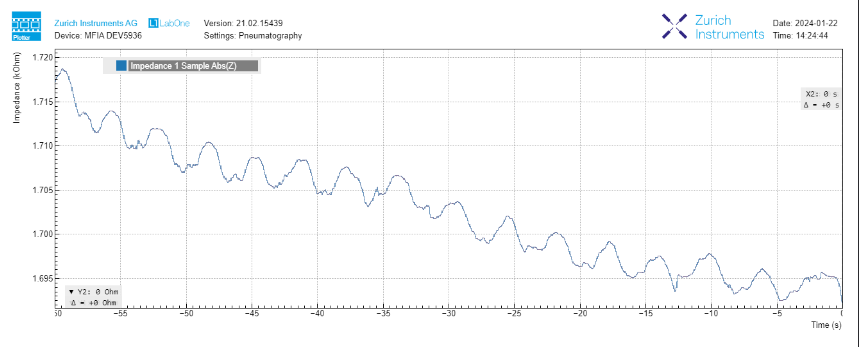
\includegraphics[width=1.2\linewidth]{figures/PlaceHolders/AgAgCl_Placeholder.png}
    \caption{AgAgCl electrodes capturing breathing}
    \label{fig:agagcl_breathing}
\end{figure}

\begin{figure}
    \centering
    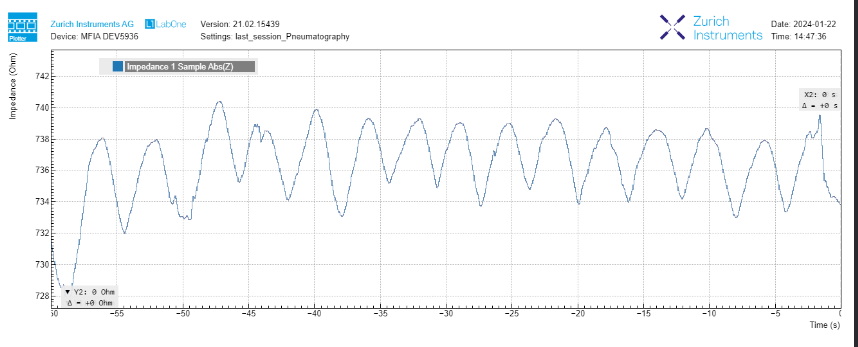
\includegraphics[width=1.2\linewidth]{figures/PlaceHolders/EDI_Gold_Placeholder.png}
    \caption{Custom, gold plated electrodes capturing breathing}
    \label{fig:edigold_breathing}
\end{figure}

\begin{figure}
    \centering
    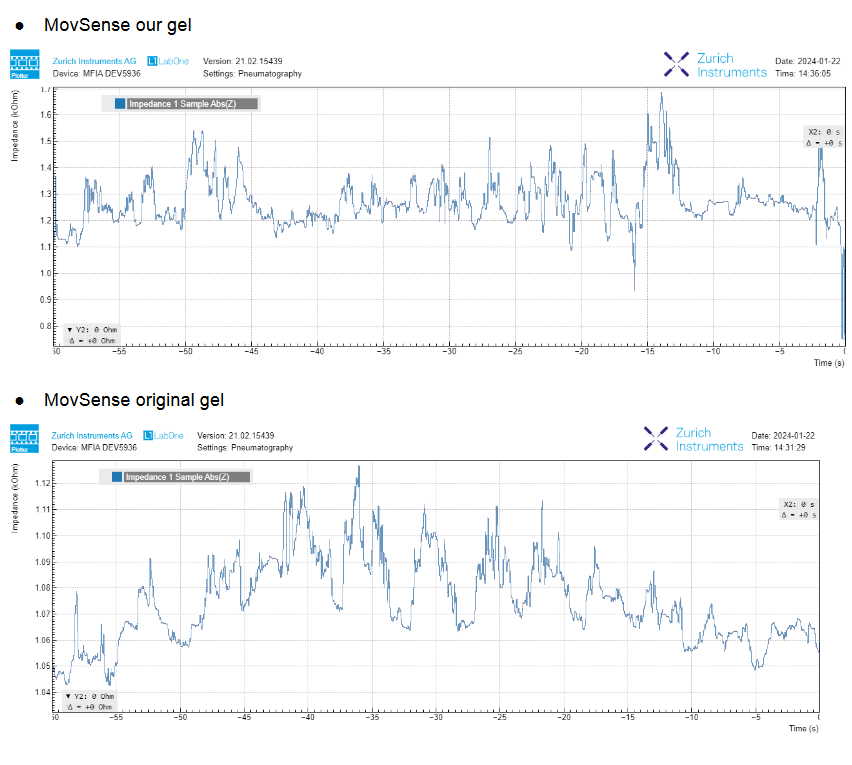
\includegraphics[width=1.2\linewidth]{figures/PlaceHolders/MovSense_Placeholder.png}
    \caption{Unknown electrodes from our shelf, we completely have no idea who is the manufacturer of those electrodes}
    \label{fig:movsense_breathing}
\end{figure}

Looking at \ref{fig:agagcl_breathing}, we see that "amplitude of inhale-exhale" is about 5 ohms, the measurement drifts from 1.72KOhm to 1.695KOhms over one minute. There is insignificant noise, about 0.1 Ohm and breathing pattern is clearly visible.

Looking at \ref{fig:edigold_breathing}, we see that "amplitude of inhale-exhale" is about 5 ohms, the measurement drifts from 734Ohm to 736Ohms over one minute. There is insignificant noise, about 0.1 Ohm and breathing pattern is clearly visible.

Looking at \ref{fig:movsense_breathing}, we are unable to see "amplitude of inhale-exhale", the measurement have no significant drift. There is drastic noise and artifacts, breathing pattern is not visible.

From those observations we can conclude that we are looking for electrodes that provides stable, low-noise, high amplitude signal.

So, to evaluate the electrodes, we will need to move from qualitative to quantitative analysis. firs of all we need to define the parameters that we are going to measure.

our proposal is to measure:
\begin{itemize}
    \item Amplitude of inhale-exhale
    \item Drift of the measurement
    \item Noise
    \item SNR
    \item Artifacts
    \item Breathing pattern visibility
    \item Heartbeat pattern visibility
    \item Muscle activity pattern visibility
    \item Skin impedance (atkartojamība)
\end{itemize}

\subsection{Methodology for benchmart development}


\subsubsection{Metrics}

Following metrics establishes a general comparison across key performance of all electrodes:
\begin{itemize}
    \item Signal-to-Noise Ratio (SNR)
    \item Durability
    \item Re-usability
    \item Sustainability
    \item Contact Impedance
    \item Skin Irritation and Comfort
    \item BER
\end{itemize}

\subsubsection{Statistical Analysis and Sample Size Determination}

To ensure the reliability of our results, we determine the minimum sample size required for each module based on the expected effect size, variability, and desired statistical power. We employ techniques such as the Analytic Hierarchy Process (AHP) for weight determination and Principal Component Analysis (PCA) for identifying the most significant metrics.

\paragraph{Sample Size Calculation}

We calculate the sample size using the formula:

\[ n = \frac{2(Z_{\alpha/2} + Z_{\beta})^2 \sigma^2}{\delta^2} \]

where \(n\) is the sample size per group, \(Z_{\alpha/2}\) is the critical value for the desired confidence level, \(Z_{\beta}\) is the critical value for the desired power, \(\sigma\) is the standard deviation, and \(\delta\) is the expected effect size.

\subsubsection{Composite Score Calculation}

A composite score is calculated for each electrode by aggregating the standardized scores across all metrics, weighted by their relative importance derived from PCA:

\[ CS = \sum_{i=1}^{n} (W_i \times S_i) \]

where \(CS\) is the Composite Score, \(W_i\) is the weight, and \(S_i\) is the standardized score for the \(i^{th}\) metric.

\subsubsection{Adjustment for Dropout Rate}

The calculated sample size is adjusted to account for potential dropouts, ensuring that the study remains adequately powered:

\[ n_{adjusted} = \frac{n}{1 - dropout\_rate} \]

\subsection{Conclusion}

This novel benchmarking protocol offers a systematic and flexible approach to electrode evaluation, enabling the comprehensive assessment of electrode performance across diverse applications. By leveraging statistical analysis and PCA for weight determination, our methodology ensures that results are both reliable and reflective of the electrodes' true capabilities in bioelectrical signal acquisition.

\section{Benchmark for Electrode Evaluation}


The objective of this section is to introduce a comprehensive and modular benchmarking protocol for evaluating the performance of different types of electrodes in bioelectrical signal acquisition. This novel approach is designed to systematically assess electrodes across multiple metrics, ensuring their suitability for a variety of medical and research applications.

\section{Experimental Design for Comprehensive Evaluation of Electrode Performance}

\subsection{Overview}
To systematically evaluate the performance of electrodes in bioelectrical signal acquisition, we have devised a set of experiments targeting key metrics: Signal-to-Noise Ratio (SNR), heart rate accuracy, impedance, transmission efficiency, bandwidth, durability, contact impedance, and energy efficiency. This section describes the experimental setup and procedures tailored to capture these metrics accurately and reliably.

\subsection{Experimental Setup}
The experimental apparatus consists of the following components:
\begin{itemize}
    \item Bioelectrical signal acquisition system capable of recording ECG, impedance pneumography, and body-coupled communication signals.
    \item Standardized electrode interface for attaching and switching between different electrodes under test.
    \item A controlled environment chamber to maintain consistent temperature and humidity levels during experiments.
    \item Calibration equipment to ensure the accuracy of signal measurements.
\end{itemize}

\subsection{Procedure}
The experimental procedure is divided into specific protocols for each metric as follows:

\subsubsection{Signal-to-Noise Ratio (SNR) and Heart Rate Accuracy}
\begin{enumerate}
    \item Attach electrodes to the standardized electrode interface connected to the signal acquisition system.
    \item Record ECG signals from a healthy volunteer at rest for a duration of 10 minutes.
    \item Calculate SNR by comparing the amplitude of the ECG signal to the background noise level.
    \item Determine heart rate accuracy by comparing the detected heart rate from the ECG recording to a reference heart rate monitor.
\end{enumerate}

\subsubsection{Impedance and Contact Impedance}
\begin{enumerate}
    \item Utilize an impedance meter to measure the impedance between two electrodes placed at a standard distance apart on a volunteer's skin.
    \item Repeat measurements under different conditions (e.g., dry skin, after application of conductive gel) to assess contact impedance.
\end{enumerate}

\subsubsection{Transmission Efficiency and Bandwidth}
\begin{enumerate}
    \item Set up a body-coupled communication experiment using two electrodes placed on opposite sides of the body.
    \item Transmit a range of frequencies through the body and measure the attenuation of the signal to determine transmission efficiency and bandwidth.
\end{enumerate}

\subsubsection{Durability and Energy Efficiency}
\begin{enumerate}
    \item Subject electrodes to a simulated wear-and-tear protocol to assess durability over time.
    \item Measure the power consumption of the electrode during continuous operation to evaluate energy efficiency.
\end{enumerate}

\subsection{Data Collection and Analysis}
Data collected from the experiments will be analyzed using statistical software to calculate each metric's values. The analysis will include descriptive statistics, comparative analysis across different electrodes, and correlation analysis to identify relationships between metrics.

\subsection{Conclusion}
This experimental design is crafted to comprehensively evaluate electrode performance across all identified metrics, ensuring a rigorous assessment of their suitability for bioelectrical signal acquisition applications. The standardized approach facilitates reproducibility and comparability of results, contributing to the advancement of electrode technology.






\input{sections/011_participants.tex}
\input{sections/012_equipment.tex}
% ... more subsections as needed
